%
%
% $Id: MD_lab.tex,v 1.14 2005/08/17 13:01:08 hteran Exp $
%
% latex MD_lab.tex ; dvips MD_lab.dvi -o MD_lab.ps; ps2pdf MD_lab.ps
%
% PACKAGES
%
\documentclass[a4paper,12pt]{article}
%\usepackage[a4paper,offset={0pt,0pt},hmargin={2cm,2cm},vmargin={2cm,2cm}]{geometry}
\usepackage{graphics}
\usepackage[dvips]{graphicx}
%% fonts
\usepackage{times}\fontfamily{ptm}\selectfont
\usepackage[activeacute,english]{babel}
%%\usepackage{t1enc}
\usepackage[latin1]{inputenc}
\usepackage{amsmath}
\usepackage{tabularx}
%
% MIS DEFINICIONES
%
\def\myname{\textbf{Hugo G. de Ter\'an}}
\title{1. Molecular Dynamics Simulations}
\author{Martin Alml\"{o}f, Martin And\'er, Sinisa Bjelic, Jens Carlsson, \\ Hugo Guti\'errez de Ter\'an, Martin Nervall, Fredrik \"{O}sterberg and Stefan Trobro}
\date{18th August 2005}
\setlength{\textheight}{9.1in}
\setlength{\textwidth}{6.0in}
\setlength{\topmargin}{-0.18in}
\setlength{\oddsidemargin}{0in}
\pagestyle{plain}
\pagenumbering{arabic}
\newcommand{\HR}{\rule{1em}{.4pt}}
\newcommand{\sctn}[1]{\section{\large #1}}
\newcommand{\subsctn}[1]{\subsection{#1}}
\newcommand{\subsubsctn}[1]{\subsubsection{#1}}
\renewcommand{\theenumi}{\alph{enumi}}
\renewcommand{\theenumii}{\arabic{enumii}}
\newcommand{\dGb}{\ensuremath{\Delta G_{\rm bind}}}
\newcommand{\dGel}{\ensuremath{\Delta G_{\rm el}}}
\newcommand{\dGvdw}{\ensuremath{\Delta G_{\rm vdW}}}
\newcommand{\qdyn}{\texttt{Qdyn5}}
\newcommand{\qprep}{\texttt{Qprep5}}
\newcommand{\qcalc}{\texttt{Qcalc5}}
\newcommand{\q}{\texttt{Q}}
\newcommand{\grep}{\texttt{grep}}
\newcommand{\sed}{\texttt{sed}}
\newcommand{\runsh}{\texttt{run{\_}Q.sh}}
\newcommand{\pymol}{\texttt{PyMOL}}

%\newcommand{\eq_lie}{}
%
% DOCUMENTO
%
\begin{document}

\maketitle

\tableofcontents

\newpage
%
%%%%%%%%%%%%%%%%%%%%%%%%%%%%%%%%%  1  %%%%%%%%%%%%%%%%%%%%%%%%%%%%%%%%%%%%%%%%%%
%


\sctn{Molecular Dynamics: theory}



The molecular dynamics (MD) simulation technique is used for solving the equations of motions for a system of particles. It also provides a useful bridge between the average {\it positions} of atoms in static  structures (xray or NMR structure, or homology model) and the measurable {\it thermodynamic properties} of chemical or biological interest.\\
%On any atomic system there are forces acting on the atoms which strive to minimize the {\it potential energy} and lead the system in a "path of least action". But on the other hand this long-range coherence is partly disrupted and fragmented by the thermal motion preventing decrease of {\it entropy}. This balance of the potential and kinetic energy result in a {\it free energy} witch if it is known can be used to calculate the abovementioned {\it properties}.
%One of the keys to the free energy is to recognize that the temperature is constant, so the kinetic contribution, due to thermal motion, can be regarded as a constant. This way any {\it free energy} change in a system is solely the result of a change in the distribution of {\it potential energy} over the atoms. We therefore need to find the distribution of positions that the atoms occupy during the thermal motion (sampling of the {\it conformational space}) and calculat the potential energy for every atom over a given static position of the system (snap shot). To keep the temperature fixed around a certain value ({\bf target temperature}) we must perform the MD simulation coupling the system to a thermal bath (see {\bf bath coupling} keyword).
The interactions of all atoms in our system are described by
classical mechanics, through the use of a {\it Force Field}. Under
the scheme of a force field, the {\it potential energy} of an atom
({\it U}) is obtained from the sum of all its bonded and non
bonded interactions. \newline
\begin{itemize}
\item The bonded interactions are applicable to bond and angle vibration and bond (torsion) rotation, plus an extra term for the so called improper torsions. This total bonded energy can be modeled as harmonic potentials (for bonds, angles and impropers) and periodic torsion angle potentials, according to equation \ref {eqnff_b}:


%\begin{equation}
%\begin{split}
\begin{equation}
\begin{array}{lll}
 U_{\rm bonded} &=&\displaystyle \sum_{\rm bonds} K_r (r - r_{eq})^2
                     + \sum_{\rm angles} K_\theta (\theta - \theta_{eq})^2 \\
                     &+&\displaystyle \sum_{\rm dihedrals} { \frac{V_n}{2} }
                                       [1 + {\rm cos}(n\phi - \gamma)]
                     + \sum_{\rm impropers} K_\xi (\xi - \xi_{eq})^2 
\end{array}
\label {eqnff_b}
%\end{split}
\end{equation}

%\end{equation}

The values of all the constants and equilibrium values in eq \ref {eqnff_b} are calibrated against experiments or quantum mechanical calculations %Equilibrium bond and angle parameters are obtained from xray structures. Force constants for angle and bond vibrations from spectroscopic data. Torsional parameters are normally obtained by quantum mechanical calculations in which the bond is restrained in different torsional angles and the energy evaluated. Bonds without spherical symmetry need an additional improper angle term because bending one atom perpendicular to the nodal plane of the {\ensuremath{\pi}} bond disrupts the {\ensuremath{\pi}} orbital overlap while bending along the nodal plane does not. The parameter {\ensuremath{\xi}} is the angle between the nodal plane and the bond between the central sp2 atom and the bending atom. Rotating the {\ensuremath{\pi}} bond also disrupts the {\ensuremath{\pi}} bond and this is modeled in the torsional term.\newline
\item In addition to the bonded interactions, pair interactions between non-bonded atoms are included in the potential energy function as electrostatic and van der Waals interactions, according to eq \ref {eqnff_nb}.

\begin{equation}
U_{\rm non-bonded} =  \sum_{i<j} \left [ \frac{A_{ij} }{R_{ij}^{12}} -
                                          \frac{B_{ij}}{R_{ij}^6}
                                 \right ]
                     + \sum_{i<j} \left [
                                          \frac{q_iq_j}{4 \pi \epsilon _{0} R_{ij}}
                                   \right ]
\label{eqnff_nb}
\end{equation}

The Lennard-Jones expression (first summation in eq \ref
{eqnff_nb}) has a repulsive term ($A_{ij} / R_{ij}^{12}$)
which models short range repulsions, while the second term
(${B_{ij} / R_{ij}^6}$) represents van der Waals or dispersion
interactions; The electrostatic equation, corresponding to the
second summation in eq \ref {eqnff_nb}, is the Coulomb interaction
for two point charges. Partial charges are obtained mainly by
quantum mechanical calculations sometimes adjusted to reproduce
dipoles and hydrogen bonds.
\end{itemize}
It is important to note that the atoms that form bonds and angles
are excluded from the non bonded interactions and that the number 
of pair interactions scale as
$N^2$ while the bonded only scale to $N$.\newline An intuitive
illustration of the mathematical and chemical meaning of each term
of the force field equations is given in figure \ref {FF}.
\newpage
%Figure 1
\begin{figure}[!ht]
\begin{center}
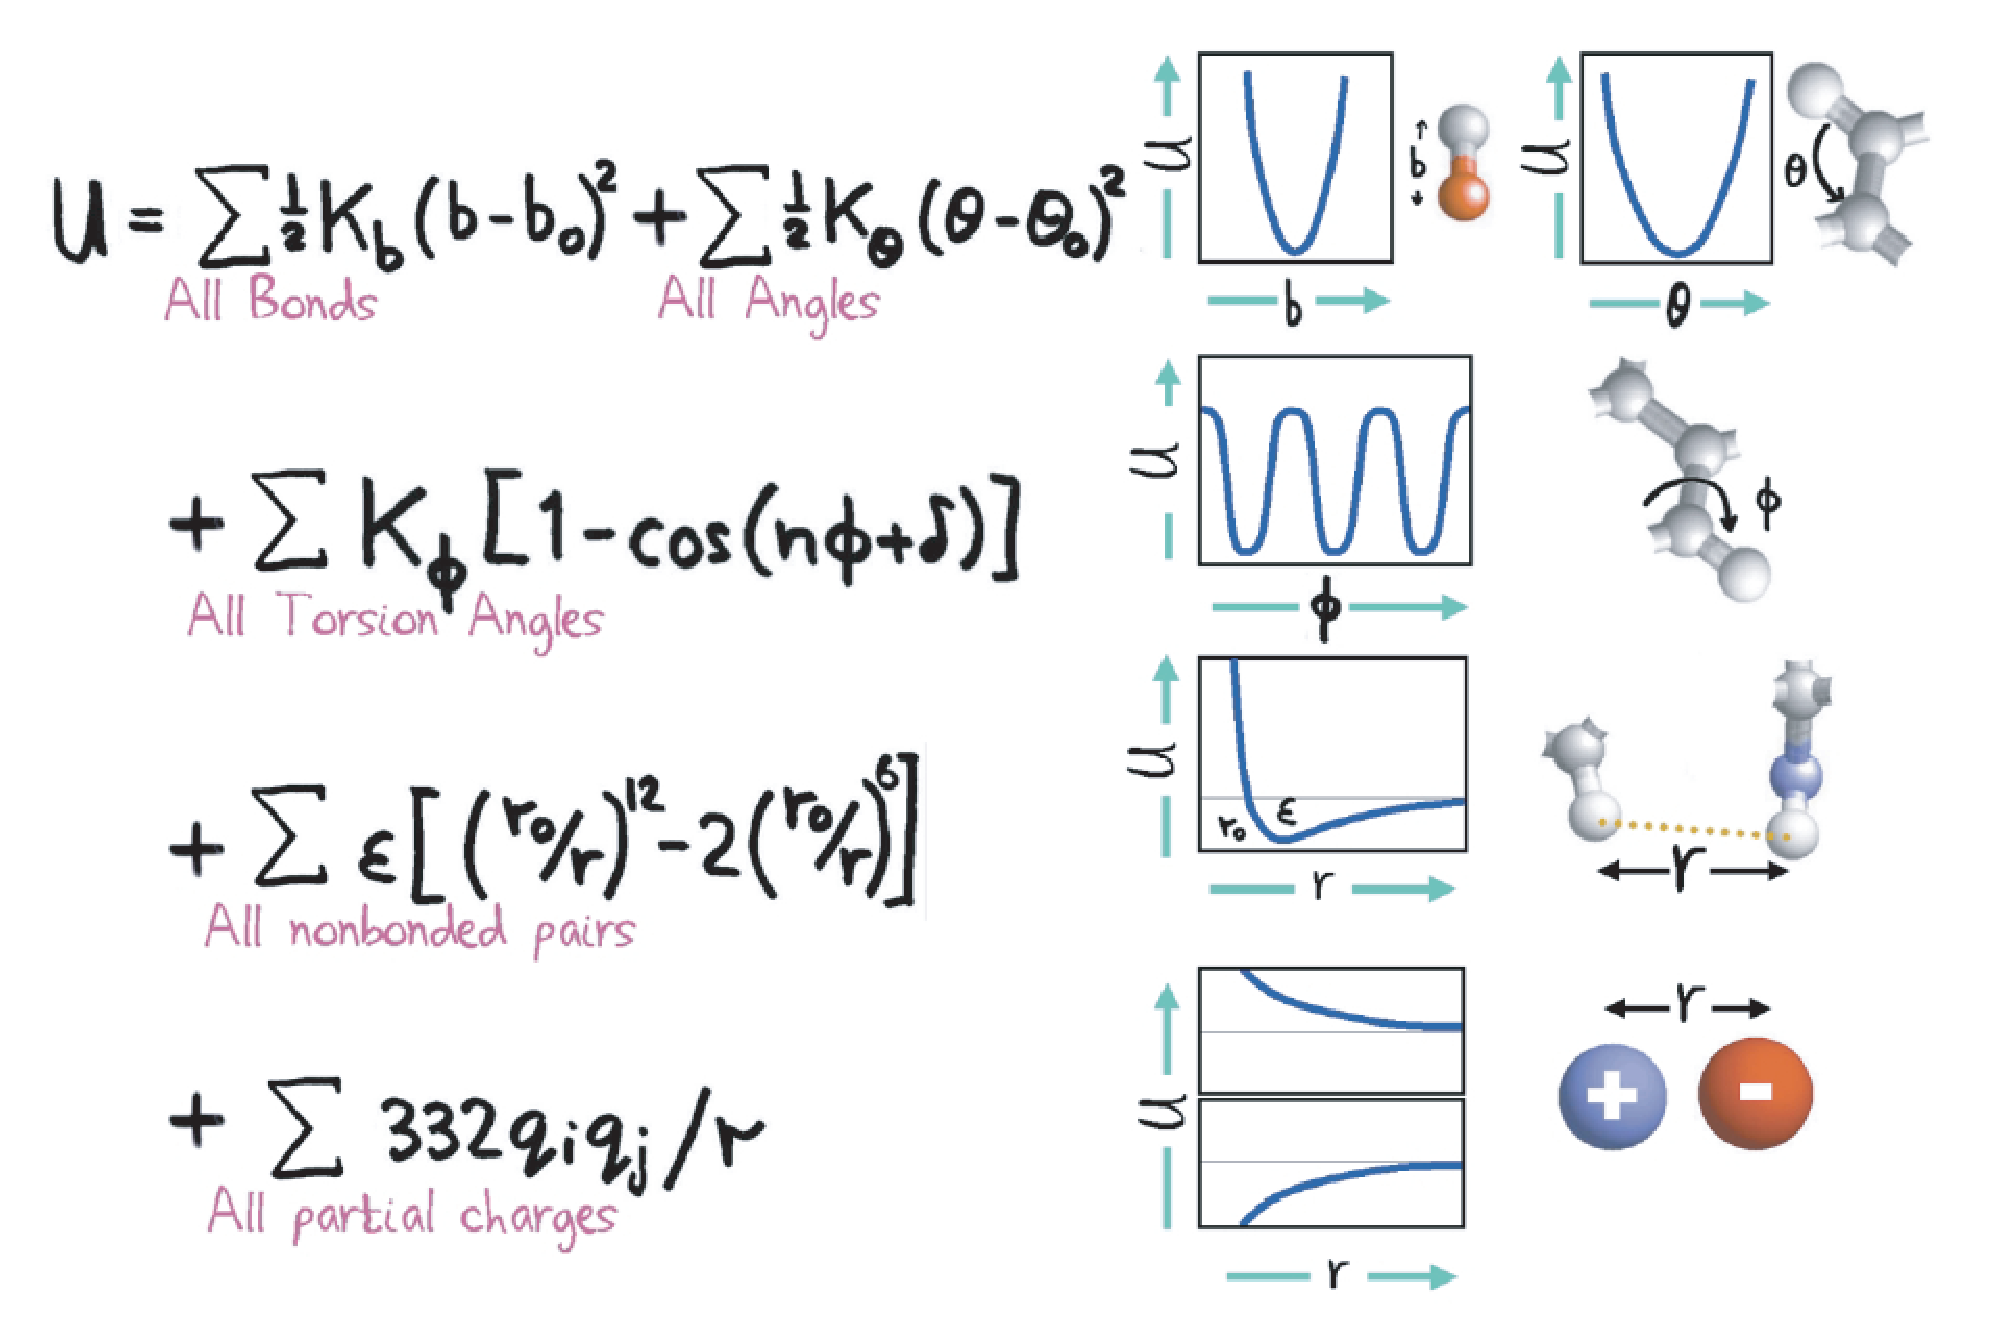
\includegraphics[width=10cm]{FF}
\caption{\label{FF} the meaning of each term in the force field equation (from M. Levitt)}
\end{center}
\end{figure}

The force field allows the atoms to be treated as point masses with forces acting between them governed by the particle positions. This is where Newtonian classical mechanics comes in to play, (see \ref{eqnw} and \ref{eqnww}).

\def\eqnw{\vec F_{\rm i} = -{\partial U_{\rm i} \over \partial r_{\rm i}}
\label {eqnw}}
\begin{equation}
\eqnw{}
\end{equation}
\def\eqnww{\vec F_{\rm i} = {m \vec a_{\rm i}}
\label {eqnww}}
\begin{equation}
\eqnww{}
\end{equation}

The time evolution of the system can be calculated according to a numerical algorithm. One such integration is the  leap-frog version of Verlet's algorithm:\\
For every atom i:
\begin{itemize}
\item   calculate $ \vec F_{\rm i}(t)$
\item   update velocity $$\vec v_{\rm i}\left(t + {\Delta t \over 2}\right) = \vec v_{\rm i} \left(t - {\Delta t \over 2}\right) + {\vec F_{\rm i}(t) \over m_{\rm i}} \cdot \Delta t$$
\item   update position $$r_{\rm i}(t+\Delta t) = r_{\rm i}(t) + \vec v_{\rm i}\left(t+{\Delta t \over 2}\right)\cdot \Delta t$$
\end {itemize}
While MD may be used for many types of applications, the goal is often to generate an ensemble of structures and energies representing thermal equilibrium. These ensembles can then be used to calculate thermodynamic properties. A few points and recommendations are worth mentioning:
\begin {itemize}
\item Starting coordinates for protein simulations are usually taken from xray structures or homology models. We need to generate a {\it topology file}, which combines the information contained in the initial PDB file (initial positions of the atoms) and the information contained in the force field for each atom.

\item The system will be modeled as spherical and centered on the chemical group of interest. Water molecules are added before the simulation to fill vacant positions and restraints are used to reproduce bulk water density and polarization near the system boundary. Atoms outside the system boundary are conformationally restrained to initial positions.
\item Charges close to the boundary should be neutralized because of the lack of dieletric screening near the boundary. Continuum corrections for energetic effects of this can be applied afterwards. These long-range effects are usually small provided that the simulation system is sufficiently large.
\item To keep the temperature fixed around a certain value ({\bf temperature} keyword) we must couple the MD simulation to a thermal bath (see {\bf bath\_coupling} keyword).
\item Starting velocities are randomly assigned (see {\bf random\_seed} keyword) from a Maxwell-Boltzman distribution for relevant mass and temperature. The velocity distribution is used to determine the temperature of the system and all velocities are then scaled to the target temperature repeatedly during the simulation. This information is stored in the so called restart files (extension {\texttt .re}), that allow us to continue a calculation from the last step or to restart a job if a crash occurs.

\item Non-bonded interactions are only calculated for atoms {\it inside} the system boundary.
\item To reduce the number of pair interactions, several approximations are introduced:
\begin {itemize}
\item For every atom {\it i} there is a cutoff (keyword {\bf cutoff}) distance for the treatment of its non bonded interactions: every possible pair {\it i,j} inside the cutoff is periodically tabulated according to a user defined interval of time steps.
\item Beyond the cutoff the electrostatic interactions are approximated through the local reaction field (keyword {\bf lrf}) approximation, in which a fourth order series expansion of the electric field, E, due to all atoms outside the cutoff is calculated. The force acting on an atom {\it i} due to the electric field is obtained by: $$\vec F_{\rm i} = \vec E_{\rm i} \cdot q_{\rm i}$$
\item All van der Waals forces outside the cutoff are ignored.
\end {itemize}
It is important to note than in any free energy calculation the
atoms whose energy will be calculated (so called Q atoms in our
programs, {\it i.e.} the ligand) do not have any of these
approximations, and they explicitly see {\it every} other atom
within the sphere of simulation. The complete list of those atoms
must be specified in a separate file, {\it e.g.} {\bf lie.fep}.
Detailed information about the variations on this file will be
given in the next practical.
\item The leap-frog algorithm calculates the velocities and positions after a given {\it time step} increment ($\Delta t$, keyword {\bf stepsize}). One decides the number of time steps, {\it n}, (keyword {\bf steps}) to be performed, and the total time of the simulation will be: $$ t_{\rm total} = n \cdot \Delta t$$
\end {itemize}


%
%%%%%%%%%%%% Methods%%%%%%%%%%%%%%%%%%%%%%%%%%%%%%%%%%%%%%%%
%
\sctn{Methods: Prepare and run the MD simulations}
In this practical you will see how to set up an MD simulation, in which the surrounding energies of a ligand, complexed with a protein, will be monitored.\\
Two parts are needed in order to run a MD simulation:
\begin {itemize}
\item {\bf Topology}: A file must be created combining the positions of the atoms and the parameters of the force field for every atom. The resulting file contains information about atom properties, connectivity, amino acid sequence, solvation model, etc \ldots
\item {\bf Input file}: It specifies the values of any variable parameter in the MD scheme: temperature, time step, number of steps, cutoff for non-bonded interactions etc \ldots
\end {itemize}
We will prepare topology and input files for the system of study, {\it cytochrome P450cam complexed with the inhibitor camphane}. The P450 enzymes, which receive this name because they absorb light maximally at 450 nm when they are complexed with CO, catalyze the hydroxylation of unactivated alkanes. This chemical reaction is used in the liver to increase the solubility of foreign substances (xenobiotic compounds), facilitating their detoxification. P450 enzymes are also involved in the synthesis of steroids and fatty acids, and in the metabolic activation of powerful carcinogens. The particular enzyme known as P450cam catalyzes specifically the hydroxylation of camphor.\\
%Figure 1
\begin{figure}[!ht]
\begin{center}
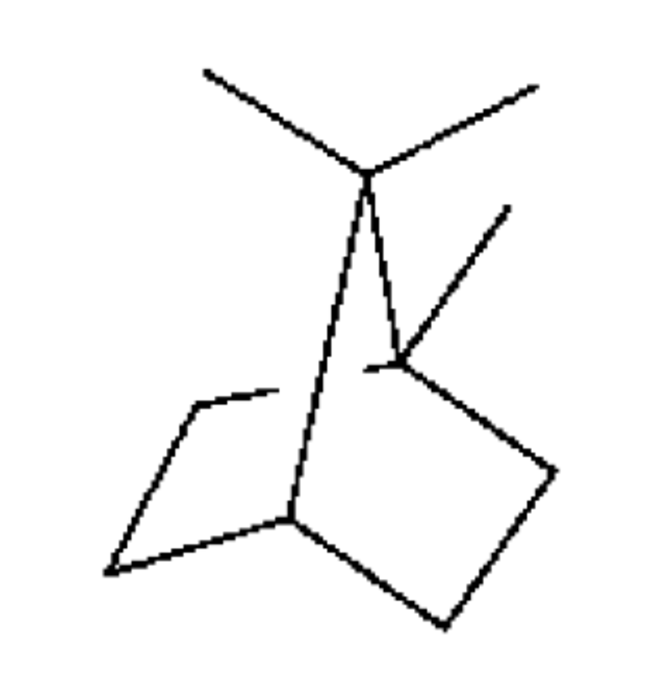
\includegraphics[width=10cm]{cam}
\caption{\label{cam} chemical structure of camphane}
\end{center}
\end{figure}
The system will be heated up and equilibrated through a series of
short MD runs. All MD simulations will be done with the modified
version of the forcefield OPLSAA, as implemented in the software
{\q}. Visual analysis will be done with the molecular modeling
program {\pymol}.

%
%%%%%%%%%%%%%%%%%%%%%%%%%%%%%%%%%%%% Protein simulation %%%%%%%%%%%%%%%%%%%%%%%%%%%%%%%%%%%
%
%
%%%%%%%%%% TOPOLOGY %%%%%%%%%%%%%%%%%%%%%%
%
\subsctn {Topology generation}
\begin {itemize}
\item Login in to your personal account and go to the working directory:
    \begin {itemize}
    \item Start your PC, and {\bf PRESS F12 BEFORE WINDOWS STARTS}.
    \item Log in to your personal account
    \item Open a UNIX terminal by right button clicking on the Desktop, and selecting "open terminal" from the pull down menu.
    \item Change to our working directory:\\
%   {\texttt cp -r /storagedir/MD .}\\
    \texttt{cd MD/P450cam}\\
    \end {itemize}


\item PDB preparation:\\
You will find the original PDB file for the P450cam-CMA complex,
under the name \texttt{6cpp.pdb}. However this file needed some
editing before using it as input for MD with our program {\q}.
Here is a list of the relevant steps that were done to generate
the suitable file \texttt{complex.pdb}, which is also in your
working directory.
    \begin {itemize}
    \item You don't need to go through these steps, but please take 5 minutes and try to understand these modifications! Open and compare the two pdb files \texttt{6cpp.pdb} and \texttt{complex.pdb}
    \item Only the ATOM and HETATM lines have been retrieved (i.e., the coordinates of the atoms).
    \item A "GAP" line is introduced between molecules, instead the default TER used by PDB convention.
    \item Only one water molecule has been conserved, which is important for the stability of the heme group, as we will see later on. For this water molecule, the hydrogens were manually added so that the orientation is optimal for hydrogen bonding to the heme group.
    \item The terminal oxygen of the last protein residue has been deleted as it will not be part of our simulations sphere of simulation
          (peptide chain termini otherwise require extra amino acid library entries).
    \item Ionizable residues (aspartic, glutamic, histidine lysine or arginine): in order to ensure a correct solvation of 
          any charged group present in the system, only those ionizable residues located in the interior of the simulation sphere 
          will be considered as charged. The OPLS residue library file (\texttt{Qoplsaa.lib}) contains both the charged 
          (ASP, GLU, HIP, LYS, ARG) and neutral (ASH, GLH, HIE, HID, LYN, ARN) version for these residues, 
          so for a given residue changing the default residue name to the charged version name on the pdb will solve the problem. After visual inspection, all ionizable residues within approximately 16 {\AA} of the C$_1$ atom of camphane were set to their ionized state, except Asp297 and Arg240. Here is a list of the charged residues in the sphere (with renumbered sequence starting at 1):\\
        \begin {itemize}
        \item ASP: 88, 173, 242
        \item GLU: 357
        \item ARG: 103, 177, 290
        \item LYS 169, 188
        \end {itemize}
    \item Note that the pdb has no hydrogens: they will be automaticaly added in the next step.
    \end {itemize}
\item Solvating the system and generating the topology:\\
The edited pdb file, named \texttt{complex.pdb} can be now
processed by the module {\qprep} of {\q} in order to solvate the
simulation sphere with TIP3P waters and write the topology file,
which contains all the necessary force field parameters. For this
step we need some files, stored in the directory
\texttt{FF{\_}Q}/:
    \begin {itemize}
    \item A library file for each molecule in the complex, with relevant information about the {\it atom names}, {\it atom types}, {\it partial charges} and {\it bonds} present in the molecule. For this particular case you have the \texttt{Qoplsaa.lib} file, with information about all the protein residues plus the water (TIP3 water model), \texttt{heme.lib} and \texttt{cma.lib}, with information about the heme group and the ligand, respectively.
    \item A parameter file, with all the  molecular mechanics parameters needed for simulate this system: {\it Van der Waals, bond stretching, angle bending, torsion and improper angle} parameters. This file is called \texttt{Qoplsaa.prm}
    \item You can take a look at the files \texttt{../FF{\_}Q/Qoplsaa.lib} and \texttt{../FF{\_}Q/Qoplsaa.prm} to get an impression of how a force field is implemented.
    \end {itemize}
Start the program {\qprep} by typing its name in the UNIX shell. The program is interactive, so it is waiting for your instructions. Type:\\
    \begin {itemize}
    \item {\texttt { readlib ../FF{\_}Q/Qoplsaa.lib}}
    \item {\texttt { readlib ../FF{\_}Q/heme.lib}}
    \item {\texttt { readlib ../FF{\_}Q/cma.lib}}
    \item {\texttt { readprm ../FF{\_}Q/Qoplsaa.prm}}
    \item {\texttt { readpdb complex.pdb}}
    \item {\texttt { addbond 5480 6383 y}} (to form the bond between the Fe atom and the S of Cys 348; 
        "y" indicates that we accept the 2.2 {\AA} bond length. Note, that the atom numbers forming the bond can be found by typing
         {\texttt { listseq}} to see the sequence and {\texttt { listres}} to see the atom numbers in a given residue)
    \item {\texttt {boundary sphere 407:C1 18}} (the centre of the 18 {\AA} radius sphere of simulation will be the central atom of the ligand, indicated by residue:atom{\_}name)
    \item {\texttt {solvate 407:C1 18 1 HOH}} (solvate with TIP3P waters the sphere of simulation)
    \item {\texttt {maketop "cma compex topology"}} (make the topology, giving a title for it)
    \item {\texttt {writetop cma.top}}
    \item {\texttt {writepdb cma{\_}top.pdb y}} (we will have a pdb of the starting coordinates of the system; "y" indicates write GAP between molecules)
    \item {\texttt {quit}}
    \end {itemize}
We have generated the topology file, \texttt{cma.top}, which will be the file used as input for the MD simulation.\\
Alternatively you can write all {\qprep} commands in a separate
file ({\it e.g.} \texttt{maketop.inp} and run {\qprep} {\texttt {<
maketop.inp > maketop.log}}, so you can carefully analyze the
output given by the program.

\item Visual analysis: \\
Typing the command \\
\texttt{pymol topology.pml} \\
you will get a nice view of the complex.
\begin {itemize}
\item Take a look at the location of the ligand, in the centre of the sphere, and the dimensions of the sphere of simulation. In practice, only atoms inside the sphere will be taken into account in the MD simulation. The definition of the size of the sphere must be a compromise between accurate description of the long-range interactions and computational effort.
\end {itemize}
\end {itemize}

%
%%%%%%%%%%% INPUT %%%%%%%%%%%%%%%%%%
%

\subsctn {Input file and running the MD simulation in {\qdyn}}
We have done half of the work. Now we need to prepare the input files for the MD simulation, with the specifications about the MD conditions.\\
Any MD simulation with explicit solvent is divided in two phases:
    \begin {itemize}
    \item Equilibration phase: The system must be equilibrated, since we start from a frozen image of the complex ({\it i.e.} crystallographic coordinates) solvated with a predefined grid of waters.
    \item Production phase: This is the part of interest, which will be later analyzed by extracting the information about the energies and other properties of interest.
    \end {itemize}
In this practical we will run the equilibration of the complex P450cam-CMA starting from the topology just generated. There will be 5 blocks of equilibration, given by the input files \texttt{eq1.inp} to \texttt{eq5.inp}. The variables of each block are outlined in the following table:\\

\begin{center}
\begin{tabularx}{\textwidth}{|c|c|c|c|c|c|X|}
\hline
Starting file & Input file & Temp (K) & Bath coupling (fs) & $\Delta$ t (fs) & {\it n} steps & Force constant ($\mathrm{{kcal \over mol} \dot{A}^{2}}$) \\
\hline
complex.top & eq1.inp & 1 & 0.2 & 0.2 & 100 & 200 \\
eq1.re & eq2.inp & 50 & 10 & 1 & 500 & 50 \\
eq2.re & eq3.inp & 150 & 10 & 1 & 500 & 25 \\
eq3.re & eq4.inp & 300 & 10 & 1 & 500 & 10 \\
eq4.re & eq5.inp & 300 & 10 & 1 & 500 & 2 \\
\hline
\end{tabularx}
\end{center}



        \begin {itemize}
        \item \texttt{eq1}: It is similar to energy minimization of the solvent and hydrogens of the solute: in this 0.02 ps run, we use a short time step and a strong coupling to the thermal bath at 1 K temperature, and heavy solute atoms restrained to their starting positions.
        \item \texttt{eq2 - eq4}: The system is gradually heated to 50, 150 and 300 K during 0.5 ps at each temperature point, with the time step increased and coupling constant relaxed. The restraints on heavy solute atoms are gradually relaxed.
        \item \texttt{eq5}: It is very similar to a production phase, but still maintaining a weak restraint on heavy solute atoms.
        \end {itemize}

A closer look to the last input file (\texttt{eq5.inp}) will tell
us exactly which keywords are used on the MD simulation of this
example:
%
%%%%%%%%%%% INPUT FILE %%%%%%%%%%%%%%%%%%%%
%
\begin{tabbing}
......................................\=........\\
\\
$[$MD$]$ \\
steps \>                    500\\
stepsize\>                  1\\
temperature\>               300.0\\
bath\_coupling\>             10\\
random\_seed\>               1231\\
shake\_solute\>              off\\
lrf\>                       on\\
\\
$[$sphere$]$ \\
shell\_force\>              10\\
shell\_radius\>             0.80\\
\\
$[$intervals$]$ \\
output\>                    50\\
\\
$[$files$]$ \\
topology\>     cma.top\\
restart\>      eq4.re\\
final\>        eq5.re\\
fep\>          lie.fep\\
\\
$[$sequence\_restraints$]$\\
1 6486 2.0 0\\
\\
..............................................\\
\end{tabbing}

Each of the titles in brackets starts a section. We are thus defining basic simulation data (section $[$MD$]$), settings for the 
simulation sphere of (section $[$sphere$]$; here we are defining a buffer region beyond 80\% of the radius where a force constant of 10.0 is applied), intervals for saving data and updating non-bonded interactions (section $[$intervals$]$), file names for input and output ($[$files$]$) and restraining sequences of atoms (section $[$sequence\_restraints$]$). In this last section, the line refers to the restraint on every heavy atom in the solute.\\
Make sure that you understand the meaning of every parameter in the input file.
Now you can launch the job. This can be easily done by running the shell script {\runsh}. Type:\\
{\texttt {tcsh run\_Q.sh qdyn eq}}\\
and wait 5 minutes until the simulation has finished.\\

\sctn {Analysis of the results}
\begin{itemize}
\item Open the last log file {\texttt {eq5.log}} with your favourite text editor (\texttt{emacs, vi}). The file has a first part in which the input data and options are read, and a second part in which the information from the trajectory is prediodically stored.
    \begin{itemize}
    \item Check that all input parameters are right and that your system is effectively neutral (look for the Total charge of system).
    \item How often (how many time steps) is the output written?
    \item Is the temperature effectively kept constant?
    \item Take a look at the register of the surrounding energies of the ligand along the trajectory. This is an example of an average property calculated through MD.
    \end {itemize}
\item You can also have a graphical feeling of the MD simulation corresponding to the "production phase" (eq5), opening the trajectory file on {\pymol} by typing:\\
\texttt{pymol trajectory.pse} \\
Once the file has been loaded click on the arrows on the
lower-right corner of the graphical interface to play the
trajectory, and you will see a small video of your run.
\begin {itemize}
\item Is the system stable?
\end {itemize}
\end {itemize}

\end{document}
